\documentclass[output=paper,colorlinks,citecolor=brown
% ,hidelinks
% showindex
]{langscibook}
\author{David Gil\affiliation{Max Planck Institute for Evolutionary Anthropology}}
\title[Hierarchical syntactic structure in Malay/Indonesian]{Hierarchical syntactic structure in Malay/Indonesian,
Between Pirahã and Had Gadya}
\abstract{This paper presents an exploration of hierarchical syntactic structure in Malay/Indonesian.  An analysis by Jackendoff and Wittenberg suggests that the Riau dialect of Indonesian may, like Pirahã, lack syntactic recursion.  This paper poses the question whether Riau Indonesian is syntactically recursive, and answers "yes and no".  In Riau Indonesian, the grammar does indeed permit the formation of sentences with arbitrarily many levels of embedding; in this respect, it appears to exhibit syntactic recursion.  However, in Riau Indonesian, the use of embedding is vanishingly rare: in a preliminary study involving comparable language registers, the frequency of embedding is found to be several orders of magnitude lesser in Malay/Indonesian than in English.  To represent the status of recursion in Malay/Indonesian, reference must be made not only to grammar but also to the ways in which speakers choose to express their conceptualization of reality: linguistic perspective.  A rough and ready indication of the propensity for a language to make use of syntactic recursion is provided by an examination of cumulative tales such as the Aramaic/Hebrew Passover song Had Gadya. Such tales occur throughout the world; however while their semantics is recursive, their syntax is often flat and concatenative, a preliminary survey suggesting that the distribution of syntactically recursive cumulative tales may be limited to a single area centered on Europe and the Middle East.  The results of this paper suggest that syntactic recursion is more likely to be found in languages spoken by communities of greater societal complexity, with Malay/Indonesian occupying an intermediate position in this respect, between Pirahã and Standard Average European.}


\IfFileExists{../localcommands.tex}{
 \addbibresource{../localbibliography.bib}
 \newcommand{\orcid}[1]{}

\usepackage{orcidlink}

\usepackage{tabularx,multicol}
\usepackage{url}
\urlstyle{same}


\usepackage{langsci-optional}
\usepackage{langsci-lgr}
\usepackage{langsci-gb4e}

% for texlive 2022
\usepackage{langsci-branding} 

% Müller


% \usepackage{biblatex-series-number-checks}

% \usepackage{eng-date}

% \usepackage{german}%% Das Buch ist nicht deutsch. Hör auf, solche Sachen zu laden


% \usepackage{tikz-dependency}
% \usepackage{tikz}
% \usepackage{tikz-qtree}

% \usepackage{hologo}

% 3_pullum.tex

% This does not work complains about recommanding epsilon
% We use a special adapted version, which is in the repro.
\usepackage{langsci-textipa}



% 8_levine

\usepackage{./styles/lg-macro2}
\usepackage{bm}
\usepackage{umoline}
\usepackage{pifont}
\usepackage{pstricks,pst-node,pst-tree}
\usepackage{ulem}
\usepackage{mathrsfs}
\usepackage{bussproofs}




%\usepackage{tikz,tikz-qtree}

%\usepackage{gb4e0}
%\noautomath

%\usepackage[letterpaper,margin=1.2in]{geometry}



% 14_kornai

%\usepackage{xypic} % seems not to be needed
% \usepackage[matrix,arrow]{xy}
%\usepackage{amsmath}
% \usepackage{subcaption}
% \usepackage{wrapfig}


 
\SetupAffiliations{output in groups = false,
                   orcid placement = after,
                   separator between two = {\bigskip\\},
                   separator between multiple = {\bigskip\\},
                   separator between final two = {\bigskip\\}
                   }

% ORCIDs in langsci-affiliations 
\definecolor{orcidlogocol}{cmyk}{0,0,0,1}
\RenewDocumentCommand{\LinkToORCIDinAffiliations}{ +m }
  {%
    \,\orcidlink{#1}%
  }


\makeatletter
\let\thetitle\@title
\let\theauthor\@author
\makeatother

\newcommand{\togglepaper}[1][0]{
   \bibliography{../localbibliography}
   \papernote{\scriptsize\normalfont
     \theauthor.
     \titleTemp.
     To appear in:
     E. Di Tor \& Herr Rausgeberin (ed.).
     Booktitle in localcommands.tex.
     Berlin: Language Science Press. [preliminary page numbering]
   }
   \pagenumbering{roman}
   \setcounter{chapter}{#1}
   \addtocounter{chapter}{-1}
}

\newbool{bookcompile}
\booltrue{bookcompile}
\newcommand{\bookorchapter}[2]{\ifbool{bookcompile}{#1}{#2}}


% Cite and cross-reference other chapters
\newcommand{\crossrefchaptert}[2][]{\citet*[#1]{chapters/#2}, Chapter~\ref{chap-#2} of this volume} 
\newcommand{\crossrefchapterp}[2][]{(\citealp*[#1]{chapters/#2}, Chapter~\ref{chap-#2} of this volume)}
\newcommand{\crossrefchapteralt}[2][]{\citealt*[#1]{chapters/#2}, Chapter~\ref{chap-#2} of this volume}
\newcommand{\crossrefchapteralp}[2][]{\citealp*[#1]{chapters/#2}, Chapter~\ref{chap-#2} of this volume}

\newcommand{\crossrefcitet}[2][]{\citet*[#1]{chapters/#2}} 
\newcommand{\crossrefcitep}[2][]{\citep*[#1]{chapters/#2}}
\newcommand{\crossrefcitealt}[2][]{\citealt*[#1]{chapters/#2}}
\newcommand{\crossrefcitealp}[2][]{\citealp*[#1]{chapters/#2}}


\newcommand{\sub}[1]{\textsubscript{\scriptsize\textrm{#1}}}

% Müller

\newcommand{\page}{}

\let\citew\citet

\def\underRevision{Revise and resubmit}

\let\textbfemph\emph

\newcommand{\todostefan}[1]{\todo[color=orange!80]{\footnotesize #1}\xspace}
\newcommand{\todosatz}[1]{\todo[color=red!40]{\footnotesize #1}\xspace}

\newcommand{\inlinetodostefan}[1]{\todo[color=green!40,inline]{\footnotesize #1}\xspace}

\newcommand{\inlinetodoopt}[1]{\todo[color=green!40,inline]{\footnotesize #1}\xspace}
\newcommand{\inlinetodoobl}[1]{\todo[color=red!40,inline]{\footnotesize #1}\xspace}

\newcommand{\itd}[1]{\inlinetodoobl{#1}}
\newcommand{\itdobl}[1]{\inlinetodoobl{#1}}
\newcommand{\itdopt}[1]{\inlinetodoopt{#1}}

\newcommand{\addpages}{\todostefan{add pages}}

%% % taken from https://tex.stackexchange.com/a/95079/18561
\newbox\usefulbox

\makeatletter
\def\getslant #1{\strip@pt\fontdimen1 #1}

\def\skoverline #1{\mathchoice
 {{\setbox\usefulbox=\hbox{$\m@th\displaystyle #1$}%
    \dimen@ \getslant\the\textfont\symletters \ht\usefulbox
    \divide\dimen@ \tw@ 
    \kern\dimen@ 
    \overline{\kern-\dimen@ \box\usefulbox\kern\dimen@ }\kern-\dimen@ }}
 {{\setbox\usefulbox=\hbox{$\m@th\textstyle #1$}%
    \dimen@ \getslant\the\textfont\symletters \ht\usefulbox
    \divide\dimen@ \tw@ 
    \kern\dimen@ 
    \overline{\kern-\dimen@ \box\usefulbox\kern\dimen@ }\kern-\dimen@ }}
 {{\setbox\usefulbox=\hbox{$\m@th\scriptstyle #1$}%
    \dimen@ \getslant\the\scriptfont\symletters \ht\usefulbox
    \divide\dimen@ \tw@ 
    \kern\dimen@ 
    \overline{\kern-\dimen@ \box\usefulbox\kern\dimen@ }\kern-\dimen@ }}
 {{\setbox\usefulbox=\hbox{$\m@th\scriptscriptstyle #1$}%
    \dimen@ \getslant\the\scriptscriptfont\symletters \ht\usefulbox
    \divide\dimen@ \tw@ 
    \kern\dimen@ 
    \overline{\kern-\dimen@ \box\usefulbox\kern\dimen@ }\kern-\dimen@ }}%
 {}}
\makeatother

% 1_intro.tex

% For the block quote:

\usepackage[most]{tcolorbox}
\definecolor{linequote}{RGB}{224,215,188}
\definecolor{backquote}{RGB}{249,245,233}
\newtcolorbox{myquote}[1][]{%
    enhanced, breakable, 
    size=minimal,
    frame hidden, boxrule=0pt,
    sharp corners,
    colback=backquote,
    #1
}

% 2_gibson.tex


% Example(s) Environments
% 12pt, No new-lines after example number is printed

\newcounter{examplectr}
\newcounter{fnexamplectr}

% Note: don't use subexamples in footnotes.

% This line is to overcome a bug in cmu-art style: it prints counter
% values to the aux file using \theaux... rather than using \the...
\def\theauxexamplectr{\theexamplectr}

\newcounter{subexamplectr}
\def\theauxsubexamplectr{\thesubexamplectr}
\def\theauxfnexamplectr{\thefnexamplectr}

\renewcommand{\theexamplectr}{\arabic{examplectr}}
% This command causes example numbers to appear without following periods

\renewcommand{\thefnexamplectr}{\roman{fnexamplectr}}
% This command causes example numbers to appear without following periods

\renewcommand{\thesubexamplectr}{\theexamplectr\alph{subexamplectr}}
% This command gives the number of an example and subexample as e.g. 1a, 2b

\newlength{\wdth}
\newcommand{\strike}[1]{\settowidth{\wdth}{#1}\rlap{\rule[.5ex]{\wdth}{1pt}}#1}

\newcommand{\exref}[1]{(\ref{#1})}
% This command puts reference numbers with parentheses
% surrounding them 

% The environment ``examples'' gives a list of examples, one on each line,
% numbered with a lower case alphabetic character
\newenvironment{examples}%
   { \vspace{-\baselineskip}
     \begin{list}%
     \textrm{\alph{subexamplectr}.}%
     {\usecounter{subexamplectr}
     \setlength{\topsep}{-\parskip}
     \setlength{\itemsep}{-2pt}
     \setlength{\leftmargin}{0.5in}
     \setlength{\rightmargin}{0in} } }%
   { \end{list}}

% The environment ``myexample'' outputs an arabic counter ``examplectr''
% surrounded by parentheses.
\newenvironment{myexample}
   { \vspace{20pt}
     \noindent
     \begin{minipage}{\textwidth}    % minipage environment disallows
                 % breaks across pages

     \refstepcounter{examplectr}     % step the counter and cause this
                 % section to be referenced by the
                 % counter ``examplectr''
     (\arabic{examplectr})}%
   { \vspace{20pt}
     \end{minipage}}

\newenvironment{myfnexample}
   { \vspace{2pt}
     \noindent
     \begin{minipage}{\textwidth}    % minipage environment disallows
                 % breaks across pages

     \refstepcounter{fnexamplectr}     % step the counter and cause this
                 % section to be referenced by the
                 % counter ``examplectr''
     (\roman{fnexamplectr})}%
   { \vspace{2pt}c
     \end{minipage}}
    
\newcommand*\circled[1]{\tikz[baseline=(char.base)]{
            \node[shape=circle,draw,inner sep=2pt] (char) {#1};}}



% 3_pullum.tex


% %%%  GKP:  I put in these pointless commands to kill off a bug elsewhere
% %%%        that tries to \newcommand \it (etc.) as \itshape (etc.), but
% %%%        fails because they haven't been defined.
% \newcommand{\it}{\relax}
% \newcommand{\bf}{\relax}
% \newcommand{\sc}{\relax}
% \newcommand{\rm}{\relax}

%%% GKP:  Two additional commands that I need
\newcommand{\data}[1]{\textit{#1}}
\newcommand{\blank}{\rule{1.2em}{0.5pt}}



% 8_levine

% ???
%\renewcommand{\emph}{\textit}
%\renewcommand{\em}{\it}

% not used \newcommand{\cites}[1]{\citeauthor{#1}'s~\citeyearpar{#1}}

% \renewcommand{\SetInfLen}{\setpremisesend{0pt}\setpremisesspace{10pt}\setnamespace{0pt}}

\newcommand{\pt}[1]{\ensuremath{\mathsf{#1}}}
\newcommand{\ptv}[1]{\ensuremath{\textsf{\textsl{#1}}}}

%\newcommand{\sv}[1]{\ensuremath{\bm{\mathcal{#1}}}}
\newcommand{\sv}[1]{\ensuremath{\mathcal{#1}}}

\newcommand{\sX}{\sv{X}}
\newcommand{\sF}{\sv{F}}
\newcommand{\sG}{\sv{G}}
%
% \renewcommand{\lex}{\SF}
% \renewcommand{\syncat}[1]{\ensuremath{\mathrm{#1}}}
% \newcommand{\syncatVar}[1]{\ensuremath{\mathit{#1}}}
%
% \newcommand{\RuleName}[1]{\textrm{#1}}
%
% \newcommand{\SemTyp}{\textsf{Sem}}
%
% \newcommand{\something}{\vdots\,\,\,\,\,\,\vdots}
%
% \newcommand{\pb}{\phantom{[}}
%
% \renewcommand{\E}{\ensuremath{\bm{\epsilon}}\xspace}
%
% \newcommand{\greeka}{\upalpha}
% \newcommand{\greekb}{\upbeta}
% \newcommand{\greekd}{\updelta}
\newcommand{\greekp}{\upvarphi}
\newcommand{\greekr}{\uprho}
\newcommand{\greeks}{\upsigma}
% \newcommand{\greekt}{\uptau}
% \newcommand{\greeko}{\upomega}
% \newcommand{\greekz}{\upzeta}
%
% % Do not do this!!!!!
% % \renewcommand{\labelenumi}{(\roman{enumi})}
%
% \newcommand{\upa}[2]{\ensuremath{\syncat{#1}|\syncat{#2}}}
% \newcommand{\dna}[2]{\upa{#2}{#1}}
%

%
% \newcommand{\Lemma}{\ensuremath{\vdots\hskip.5cm\vdots}\noLine}
%
% \newcommand{\la}{\ensuremath{\langle}}
% \newcommand{\ra}{\ensuremath{\rangle}}
%
% \renewcommand{\I}{\iota}
%
% \renewcommand{\sem}{\ensuremath}
%
% \newcommand{\LemmaShort}{\ensuremath{\vdots\hskip.2cm\vdots\hskip.2cm\vdots}\noLine}
% \newcommand{\LemmaShortAlt}{\ensuremath{\vdots\hskip.2cm\vdots}}
%
%
% \newcommand{\NoSem}{%
% \renewcommand{\LexEnt}[3]{##1; \syncat{##3}}
% \renewcommand{\LexEntTwoLine}[3]{\renewcommand{\arraystretch}{.8}%
% \begin{array}[b]{l} ##1;  \\ \syncat{##3} \end{array}}
% \renewcommand{\LexEntThreeLine}[3]{\renewcommand{\arraystretch}{.8}%
% \begin{array}[b]{l} ##1; \\ \syncat{##3} \end{array}}}
%
%
% \newcommand{\NoSemVar}{%
% \renewcommand{\LexEnt}[3]{##1; \syncat{##3}}
% \renewcommand{\LexEntTwoLine}[3]{\renewcommand{\arraystretch}{.8}%
% \begin{array}{l} ##1;  \\ \syncat{##3} \end{array}}
% \renewcommand{\LexEntThreeLine}[3]{\renewcommand{\arraystretch}{.8}%
% \begin{array}{l} ##1; \\ \syncat{##3} \end{array}}}
%
% \newcommand{\vs}{\raisebox{.05em}{\ensuremath{\upharpoonright}}}
%
% \newcommand{\AXX}[1]{\raisebox{-7mm}{\ensuremath{#1}}}
%
% \newcommand{\hypml}[2]{\left[\!\!#1\!\!\right]^{#2}}
%
% \newcommand{\alt}[2]{$\left\{\begin{array}{c}
% \hskip-.7ex\textrm{#1}\hskip-.7ex \\
% \hskip-.7ex\textrm{#2}\hskip-.7ex
%         \end{array}
% \right\}$}
%
% \newcommand{\altalt}[2]{\{#1/#2\}}
%
%
%
% \newcommand{\altt}[3]{$\left\{\begin{array}{c}
% \hskip-.7ex\textrm{#1}\hskip-.7ex \\
% \hskip-.7ex\textrm{#2}\hskip-.7ex \\
% \hskip-.7ex\textrm{#3}\hskip-.7ex
% \end{array}
% \right\}$}
%
% \newcommand{\alttt}[4]{$\left\{\begin{array}{c}
% \hskip-.7ex\textrm{#1}\hskip-.7ex \\
% \hskip-.7ex\textrm{#2}\hskip-.7ex \\
% \hskip-.7ex\textrm{#3}\hskip-.7ex \\
% \hskip-.7ex\textrm{#4}\hskip-.7ex
% \end{array}
% \right\}$}
%
%
% %%%%for bussproof
%
% \def\defaultHypSeparation{\hskip0.1in}
% \def\ScoreOverhang{0pt}
%
%
% %%\newcommand{\MultiLine}[1]{\renewcommand{\arraystretch}{.8}%
% %%\ensuremath{\begin{array}{l} #1 \end{array}}}
%
\newcommand{\MultiLine}[1]{\renewcommand{\arraystretch}{.8}%
\ensuremath{\begin{array}[b]{l} #1 \end{array}}}

%
%
% \newcommand{\MultiLineMod}[1]{%
% \ensuremath{\begin{array}[t]{l} #1 \end{array}}}
%
%
% %%%%%\AFourMargin
% %%\JLSubmissionMargin
%
% %%\setlength\topmargin{-1cm}
% %%\setlength\textheight{23cm}
% %%%%%\setlength\textwidth{13.5cm}
%
% %\setstretch{1.2}
%
% % not used \newcommand{\hyp}[2]{[ #]^{#2}}
%
\newcommand{\LexEnt}[3]{#1; \ensuremath{#2}; \syncat{#3}}
%
% \newcommand{\LexEntTwoLine}[3]{\renewcommand{\arraystretch}{.8}%
% \begin{array}[b]{l} #1; \\ \ensuremath{#2};  \syncat{#3} \end{array}}
%
% \newcommand{\LexEntThreeLine}[3]{\renewcommand{\arraystretch}{.8}%
% \begin{array}[b]{l} #1; \\ \ensuremath{#2}; \\ \syncat{#3} \end{array}}
%
%
% \newcommand{\LexEntFiveLine}[5]{\renewcommand{\arraystretch}{.8}%
% \begin{array}{l} #1 \\ #2; \\ \ensuremath{#3} \\ \ensuremath{#4}; \\ \syncat{#5} \end{array}}
%
%
% \newcommand{\LexEntFourLine}[4]{\renewcommand{\arraystretch}{.8}%
% \begin{array}{l} \pt{#1} \\ \pt{#2}; \\ \syncat{#4} \end{array}}
%
% \newcommand{\ManySomething}{\renewcommand{\arraystretch}{.8}%
% \raisebox{-3mm}{\begin{array}[b]{c} \vdots \,\,\,\,\,\, \vdots \\
% \vdots \,\,\,\,\,\, \vdots \end{array}}}
%
%
% \newcommand{\lemma}[1]{\renewcommand{\arraystretch}{.8}%
% \begin{array}[b]{c} \vdots \,\,\,\,\,\, \vdots \\ #1 \end{array}}
%
% \newcommand{\lemmarev}[1]{\renewcommand{\arraystretch}{.8}%
% \begin{array}[b]{c} #1 \\ \vdots \,\,\,\,\,\, \vdots \end{array}}
%
% \newcommand{\p}{\ensuremath{\upvarphi}}
%
% \newcommand{\Not}{\leavevmode\llap{\textbf{\smc{NOT:}} }}
%
% \newcommand{\Conj}{\fs{\bsp{\mathit{X}}{\mathit{X}}}{\mathit{X}}}
% \newcommand{\ConjY}{\fs{\bsp{\mathit{Y}}{\mathit{Y}}}{\mathit{Y}}}
% \newcommand{\sameLE}{\dna{(\upa{(\upa{S}{\mathit{X}})}{NP})}{(\upa{S}{\mathit{X}})}}
%
% \newcommand{\derivcenter}[2][1.1]{%
% \SetInfLen
% \attop{\vskip3ex
% \resizebox{#1\linewidth}{!}{\hskip-#1in
% #2}}}
%
% \newcommand{\derivcenterAlt}[2][.98]{%
% \SetInfLen
% \attop{\vskip3ex
% \resizebox{#1\linewidth}{!}{\hskip-#1in \hskip.5in
% #2}}\vspace{.5ex}}
%
% \renewcommand{\O}{\circ}  Do not recommand!
\newcommand{\BobsO}{\circ}
%
% \newcommand{\derivcenterMod}[2][1.1]{%
% \renewcommand{\LexEntThreeLine}[3]{\renewcommand{\arraystretch}{.8}%
% \raisebox{.4ex}{\ensuremath{\begin{array}{l} ##1; \\ \ensuremath{##2}; \\ \syncat{##3} \end{array}}}}
% \SetInfLen
% \attop{\vskip3ex
% \resizebox{#1\linewidth}{!}{\hskip-#1in
% #2}}}
%
%
% \newcommand{\shortarrow}{\xspace\hskip-1.2ex\scalebox{.5}[1]{\ensuremath{\bm{\rightarrow}}}\hskip-.5ex\xspace}
%
% \newcommand{\SemInt}[1]{\mbox{$[\![ \textrm{#1} ]\!]$}}
%
% \def\maru#1{{\ooalign{\hfil
%   \ifnum#1>999 \resizebox{.25\width}{\height}{#1}\else%
%   \ifnum#1>99 \resizebox{.33\width}{\height}{#1}\else%
%   \ifnum#1>9 \resizebox{.5\width}{\height}{#1}\else #1%
%   \fi\fi\fi%
% \/\hfil\crcr%
% \raise.167ex\hbox{\mathhexbox20D}}}}
%
\newcommand{\HypSpace}{\hskip-.8ex}
\newcommand{\RaiseHeight}{\raisebox{2.2ex}}
% \newcommand{\RaiseHeightLess}{\raisebox{1ex}}
%
% \newcommand{\fW}{\ensuremath{\mathfrak{W}}}
%
\newcommand{\ThreeColHyp}[1]{\RaiseHeight{\Bigg[}\HypSpace#1\HypSpace\RaiseHeight{\Bigg]}}
% \newcommand{\TwoColHyp}[1]{\RaiseHeightLess{\Big[}\HypSpace#1\HypSpace\RaiseHeightLess{\Big]}}
%
%
% %\newcommand{\maskref}[1]{\textsl{\textbf{[reference omitted for refereeing]}}}
% \newcommand{\maskref}[1]{#1}
%
% \newcommand{\DerivSize}{\small}
% \newcommand{\AppDerivSize}{\footnotesize}
%
% \renewcommand{\sem}{\ensuremath}


% \newcommand{\greekp}{{\color{green}π}}
% \newcommand{\greekr}{{\color{green}\textrho}}
% \newcommand{\greeks}{{\color{green}\textsigma}}
\newcommand{\ptfont}[1]{\texttt{#1}}                % what does ptfont do? Where is it defined?
                                % Question
%\newcommand{\ptfont}{\ttfamily}

%\newcommand{\grey}{\color{gray}}
\newcommand{\grey}[1]{\colorbox{mycolor}{#1}}
\definecolor{mycolor}{gray}{0.8}

\newcommand{\gap}{\longrule}
\newcommand{\gp}{\gap}
\newcommand{\vs}{\raisebox{.05em}{\ensuremath{\upharpoonright}}}
% \newcommand{\sub}[1]{\textsubscript[#1]}
\newcommand{\E}{\emph}
\newcommand{\B}{\textbf}
\newcommand{\f}{{\color{green}f}}  % Question what does f do? It does not have any output in the
                                % original PDF
%\newcommand{\Lemma}{{\color{pink}Lemma}}
\newcommand{\Lemma}{\ensuremath{\vdots\hskip.5cm\vdots}\noLine}

%\newcommand{\calP}{{\color{pink}calP}} % Sebastian
\newcommand{\calP}{\ensuremath{\mathcal{P}}}


\newcommand{\maru}[1]{\ooalign{\hfil#1\/\hfil\crcr
      \raise.05ex\hbox{\LARGE\mathhexbox20D}}}


%\newcommand{\sem}[2][M\!,g]{\mbox{$[\![ \mathrm{#2} ]\!]^{#1}$}}
\newcommand{\sem}{\ensuremath}

%
\newcommand{\trns}[1]{\textbf{#1}\xspace}

\newcommand{\bs}{{\textbackslash}}
\newcommand{\bsl}{{\bs}}


\newcommand{\fb}[1]{\textsubscript{#1}}

\newcommand{\syncat}[1]{\ensuremath{\mathrm{#1}}}
\newcommand{\term}[1]{\textit{#1}}
\newcommand{\LemmaAlt}{\ensuremath{\vdots\hskip.5cm\vdots}}

%\renewcommand{\O}{ø}

 %% hyphenation points for line breaks
%% Normally, automatic hyphenation in LaTeX is very good
%% If a word is mis-hyphenated, add it to this file
%%
%% add information to TeX file before \begin{document} with:
%% %% hyphenation points for line breaks
%% Normally, automatic hyphenation in LaTeX is very good
%% If a word is mis-hyphenated, add it to this file
%%
%% add information to TeX file before \begin{document} with:
%% %% hyphenation points for line breaks
%% Normally, automatic hyphenation in LaTeX is very good
%% If a word is mis-hyphenated, add it to this file
%%
%% add information to TeX file before \begin{document} with:
%% \include{localhyphenation}
\hyphenation{
    par-a-digm
}

\hyphenation{
    par-a-digm
}

\hyphenation{
    par-a-digm
}

 \boolfalse{bookcompile}
 \togglepaper[23]%%chapternumber
}{}

\graphicspath{ {./figures/} }

\begin{document}
\maketitle

\section{Introduction}
Dan Everett's main claim to fame, among linguists at least, is describing a language, Pirahã, arguably lacking many of the supposedly necessary design features of contemporary human language, such as numerals and quantifiers, colour terms, reference to things and events outside immediate experience, and of course, the cherry on the top, syntactic recursion \citep{everett2005cultural}. Meanwhile, on the other side of the world, far from the spotlight, I have worked on describing the Riau dialect of Indonesian, which turns out to be lacking in a rather different set of core features, including words, distinct open syntactic categories, systematic encoding of thematic roles, and a grammaticalized distinction between attribution and predication \citep{gil2005word,gil2006intonation,gil2012predication,gil2013riau, gil2017isolating, gil2020isolating}. This festschrift to Dan Everett presents an ideal opportunity to indulge in a contrastive analysis of the two languages — to see what happens when Pirahã meets Riau Indonesian. With neither the time nor the space to deal with the two languages in their entireties, I shall cut to the chase and focus on that most renowned feature associated with Dan Everett's work, namely syntactic recursion.

\section{Is Riau Indonesian Syntactically Recursive?}
In earlier conversations, Dan Everett (p.c.) suggested that Riau Indonesian may also be a language lacking in syntactic recursion. However, in his writings, for example \citet{futrell2016corpus}, \citet{everett2017grammar}, he makes it clear that he bases this position on the analyses proposed by \citet{jackendoff2014syntax, jackendoff2017linear}, who characterize Riau Indonesian as instantiating their class of Multi-Word Phrase Grammars, in which words group together to form phrases, and phrases group together to form utterances, but without any possibilities for syntactic recursion. However, \cite{jackendoff2014syntax, jackendoff2017linear} themselves base their analysis on my own descriptions, so let us now take a look at what I have written on this score, and also some additional facts that I have not yet had the opportunity to describe in print. Spoiler alert: The answer to the question ``Is Riau Indonesian syntactically recursive?'' is ``Yes and no''.
Indeed, in Riau Indonesian, the grammar permits the formation of sentences such as the following:

\ea\label{ex:gil:1}
\gll Ali	pukul	orang	yang	suka	anjing	yang	kejar	anak\\
 Ali	hit	person	\textsc{prtc}	like	dog	\textsc{prtc}	chase	child\\
\glt 'Ali hit the person who likes the dog that chased the child.'
\z

Moreover, if one really wants to, one can go on adding relative clauses at the end of the construction indefinitely. So in this respect, Riau Indonesian is clearly syntactically recursive, like English, not like Pirahã.
In previous work, my focus was largely on the grammar of simple word combinations, such as Ayam makan (chicken eat), and thus, while making it clear that combinations of words can be grouped together to form ever larger combinations, this particular aspect of Riau Indonesian was not emphasized. This, then, is the appropriate time to redress the balance, by presenting an explicit analysis of hierarchical structure in Riau Indonesian. A syntactic analysis of sentence \REF{ex:gil:1}, following the theoretical framework laid out in \citet{gil2000syntactic}, is presented in Figure \ref{fig:gil:fig1}.

\begin{figure}
\centering
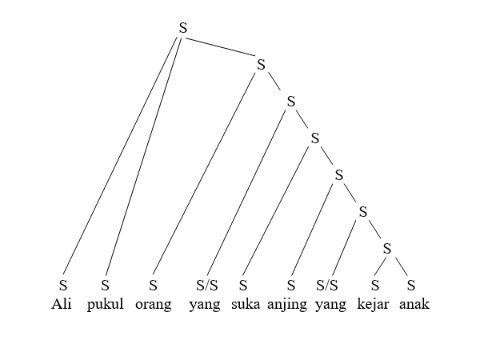
\includegraphics[width=0.8\textwidth]{gil_figure1.png}
\caption{\label{fig:gil:fig1}Syntactic Structure of \REF{ex:gil:1}}
\end{figure}

In Riau Indonesian, almost all words belong to the single open syntactic category S, for Sentence; this includes, among others, words denoting things, such as \emph\{anak\} 'child', as well as words denoting activities, such as \emph\{kejar\} 'chase'. The combination of the two, as in \emph\{kejar anak\} above, is thus an instance of sentential coordination. Similarly, complex Ss may combine with other simple or complex Ss to yield hierarchical structures such as that in Figure \ref{fig:gil:fig1}. While most words belong to the category S, a handful of grammatical items belong to a closed class, S/S, whose name, following the conventions of categorial grammar, stipulates that they cannot occur on their own but rather must combine with Ss to yield superordinate Ss. Figure \ref{fig:gil:fig1} contains two occurrences of the S/S word yang; in one case it combines with the S expression \emph\{kejar anak\} to yield a superordinate S expression yang kejar anak, while in the other case it takes the S expression \emph\{suka anjing yang kejar anak\} to yield a superordinate S expression \emph\{yang suka anjing yang kejar anak\}. As suggested by the above, the syntax of Riau Indonesian is thus fully recursive, allowing for hierarchical syntactic structures of arbitrary depth.

As shown in Figure \ref{fig:gil:fig2} below, the basic compositional semantics of sentence \REF{ex:gil:1} makes reference to a hierarchical structure that is completely isomorphic to that of its syntax:

\begin{figure}
\centering
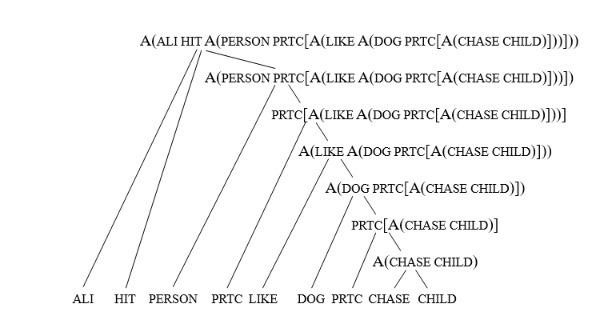
\includegraphics[width=0.8\textwidth]{gil_figure2.png}
\caption{\label{fig:gil:fig2}Semantic Structure of ¨}
\end{figure}

As represented in Figure \ref{fig:gil:fig2}, the semantics of sentence \REF{ex:gil:1} makes reference to two operators. First and foremost is the Association Operator A, which underlies the overwhelming majority of the compositional semantics. In its polyadic guise, illustrated above, it is a generalization of the monadic Association Operator, familiar as a semantic representation for genitive markers and various other possessive and associative constructions in many languages. Applying to two meanings, X and Y, A(X,Y) simply means 'entity associated with X and Y', or 'something to do with X and Y'. For example, in the above representation, A(CHASE CHILD(, the meaning of kejar anak, means 'entity associated with chase and child'; among many other things, it is unspecified for a variety of semantic categories such as number, definiteness, tense-aspect, and thematic role assignment (e.g. whether the child is the agent or patient of the chasing). The second operator is the Participant Operator \textsc{prtc}, which, when applied to a meaning X, creates a new meaning \textsc{prtc}(X), picking out a participant in the semantic frame of X. The Participant Operator underlies the semantic representation of grammatical markers in several languages, which, under alternative analyses, are sometimes characterized as relativizers, nominalizers or reifiers. For example, in the above representation, \textsc{prtc}[A(CHASE CHILD)[ denotes a participant associated with the entity associated with chase and child, without any further specification of thematic role (i.e. whether it is the agent, the patient, or perhaps some other thematic role). The above analysis captures the fact that sentence \REF{ex:gil:1} is massively underspecified with respect to categories such number, definiteness, tense-aspect and thematic roles, with respect to which the English translation in \REF{ex:gil:1}, 'Ali hit the person who likes the dog that chased the child', is just one of myriad alternative available translations.

The above analysis may be contrasted with the alternative approach proposed by \citet{jackendoff2014syntax,jackendoff2017linear}. One feature shared by both approaches is monocategoriality, the claim that Riau Indonesian has but a single open syntactic category.  However, there are at least two significant differences between the two approaches.  One pertains to the semantics, with respect to which \citet{jackendoff2014syntax,jackendoff2017linear} propose a more conventional analysis, based not on the Association Operator but rather on the familiar predicate-argument relationship.  However, it is the second difference between the two approaches, pertaining to the syntax, that is of relevance to us here.  In contrast to the above analysis, \citet{jackendoff2014syntax,jackendoff2017linear} assign Riau Indonesian to their class of Multi-Word Phrase Grammars, whose structures are flatter and non-recursive, making reference to just three categories, W(ord), P(hrase) and U(tterance).  In fact, in their view, even these categories are more appropriately viewed as phonological, or prosodic, rather than syntactic.  An analysis of sentence \REF{ex:gil:1} in accordance with \citet{jackendoff2014syntax,jackendoff2017linear}, whose approach is presented in Figure \ref{fig:gil:fig3}.

\begin{figure}
\centering
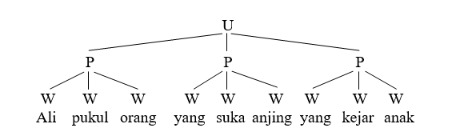
\includegraphics[width=0.8\textwidth]{gil_figure3.png}
\caption{\label{fig:gil:fig3}Semantic Structure of \REF{ex:gil:1}}
\end{figure}

In accordance with the analysis in Figure \ref{fig:gil:fig3}, sentence \REF{ex:gil:1} does not exhibit multiple layers of hierarchical structure; instead it consists of a flat sequence of phrases, each consisting of a flat sequence of words.  For \citet{jackendoff2014syntax,jackendoff2017linear}, the obviously hierarchical nature of sentence \REF{ex:gil:1} is a fact about its semantics, not its syntax.

How might one adjudicate between the alternative analyses of sentence \REF{ex:gil:1} as represented in Figures \ref{fig:gil:fig1} and \ref{fig:gil:fig3} respectively?  Given the flexibility of Riau Indonesian syntax as described in my earlier publications, Jackendoff and Wittenberg had good prima facie reason to invoke Occam's Razor and assign Riau Indonesian to their class of Multi-Word Phrase Grammars, entailing analyses such as that represented in Figure \ref{fig:gil:fig3}.  Thus, with reference to Riau Indonesian, Jackendoff and Wittenberg (p.c.) argue that:

\begin{quote}
     \ldots . its grammar relates the semantic structure of sentences directly to linear order and prosodic constituency within phonology, without the intervention of syntax.  This sort of grammar relies on principles such as Behaghel’s First Law  \ldots . Agent precedes Patient, and Modifier precedes (or follows) Modified.  None of these requires syntax  \ldots .
\end{quote}
Nevertheless, additional evidence suggests that the flat structures of Multi-Word Phrase Grammars are insufficient to account for the totality of facts pertaining to the syntax of Riau Indonesian.

As alluded to in the above passage by Jackendoff and Wittenberg (p.c.), one of the core characteristics of Riau Indonesian sentence structure is the extent, greater than in many other languages, to which it upholds Behaghel's First Law, which, paraphrasing slightly, states that expressions whose meanings are closer to each other in conceptual space tend to occur closer to each other within the syntactic structure of the sentence \citep{behaghel1932deutsche}.  One manifestation of the strongly Behaghelian nature of Riau Indonesian is the relative infrequency with which expressions occur outside of their ``expected'' positions — the kinds of constructions that, within some theoretical frameworks, are often for in terms of various kinds of movement rules.  In the case at hand, Behaghel's First Law provides clear cut and unambivalent motivation for several of the intermediate levels of syntactic structure posited by the analysis in Figure \ref{fig:gil:fig1} but absent from the flatter structure posited by the analysis in Figure \ref{fig:gil:fig3}.

Consider, for example, the substring of words \emph{anjing yang kejar anak} (dog \textsc{prtc} chase child) in \REF{ex:gil:1}, which forms a constituent in Figure \ref{fig:gil:fig1} but not Figure \ref{fig:gil:fig3}.  This constituency reflects the fact that these four words are close to each other semantically, \emph{anjing} and \emph{anak} being participants in the activity denoted by kejar.  In doing so, it makes correct predictions about possible reorderings of the words in \REF{ex:gil:1}.  For example, it correctly predicts that \emph{anjing yang kejar anak} can be moved, as a single chunk, to the beginning of the sentence, as in (2) below:

\ea
\gll Anjing	yang	kejar	anak	Ali	pukul	orang	yang	suka\\
 dog	PRTC	chase	child	Ali	hit	person	PRTC	like	\\
\glt 'The dog that chased the child, Ali hit the person who likes it.'
\z

Conversely, it also correctly predicts that yang suka anjing, a constituent in Figure \ref{fig:gil:fig3} but not Figure \ref{fig:gil:fig1}, cannot be moved to the beginning of the sentence, as in (3) below, without a massive change in meaning:

\ea
\gll Yang	suka	anjing	Ali	pukul	orang	yang	kejar	anak\\
 \textsc{prtc}	like	dog	Ali	hit	person	PRTC	chase	anak\\
\glt 'As for the one who likes the dog, Ali hit the person who chased the child.' \\
*	Ali hit the person who likes the dog that chased the child.' [= \REF{ex:gil:1}]
\z

As indicated above, the interpretation associated with sentence \REF{ex:gil:1} is completely unavailable in (3).  More dramatically, the hierarchical syntactic structure of Figure \ref{fig:gil:fig1} predicts the total unacceptability, salva veritate, of various random reshufflings of the words in \REF{ex:gil:1} such as in (4) below:

\ea
\gll Orang	pukul	anjing	yang	suka	anak	yang	kejar	Ali \\
    person	hit	dog	PRTC	like	child	PRTC	chase	Ali\\
\glt 		'A person hit the dog that likes the child who chased Ali.' \\
*	Ali hit the person who likes the dog that chased the child.' [= \REF{ex:gil:1}]
\z

Again, the interpretation associated with sentence \REF{ex:gil:1} is completely unavailable in (4).  Thus, as shown above, Riau Indonesian has nothing of the freedom of, say, a language like Warlpiri, for which \citet{hale1979position, hale1983warlpiri} posits a flat ``W-star'' grammar. Instead, the strongly Behaghelian nature of Riau Indonesian, compensating for its flexibility and indeterminacy in various other domains, provides strong support for hierarchical syntactic structures of the kind represented in Figure \ref{fig:gil:fig1}, and in doing so for the presence of syntactic recursion in Riau Indonesian.

Jackendoff and Wittenberg (p.c.) propose to account for facts similar to these by positing a ``Contiguity Condition'', whose effect is to ensure that what they call ``semantic constituents'' must be expressed by contiguous strings of words.  For example, in order to account for the inseparability of the string \emph{anjing yang kejar anak}, as evidenced in \REF{ex:gil:1} - (4) above, they would invoke the Contiguity Condition to ensure that the semantic constituent A(DOG \textsc{prtc}[A(CHASE CHILD)], is realized by a contiguous string of words.  Crucially, according to Jackendoff and Wittenberg, such strings do not form syntactic constituents; rather, they are semantic constituents that are then mapped onto phonological ones.  Their analysis is in accordance with their general agenda, which is to avoid reference to syntax unless the phenomenon under question cannot be accounted for with reference to either semantics or phonology.  While in general I am supportive of their agenda, in the case at hand there is an obvious problem, namely, their assumption that contiguity is a fact about phonology.  While in some cases, indeed, contiguous words may interact phonologically, for example by forming an intonational phrase, this is not true more generally; for example, in \REF{ex:gil:1}, the string \emph{anjing yang kejar anak}, argued in (2) to form a syntactic constituent, does not constitute a complete intonational phrase.  Rather, contiguity must be viewed as a syntactic property, indeed perhaps the most quintessential one, pertaining to what syntax is all about, namely, the bringing together of expressions in order to constitute larger expressions.  Thus, pace Jackendoff and Wittenberg, the strongly Behagelian nature of Riau Indonesian, as exemplified by the above examples, does indeed support the kind of hierarchical syntactic structure illustrated in Figure \ref{fig:gil:fig1}, and in so doing also the presence of syntactic recursion in Riau Indonesian.

With respect to the presence of syntactic recursion, then, Riau Indonesian is more like English than like Pirahã.  But still, this is only half the story.  A more fully adequate account of recursion in Riau Indonesian must acknowledge the fact that sentences such as in \REF{ex:gil:1} are highly artificial, and that nobody actually speaks that way.  Exactly what it means to say that nobody speaks that way is taken up in the next section.

\section{Linguistic Perspective (Or, What it Means to Know a Language)}
Among the scholars who have addressed the broader implications of my analysis of Riau Indonesian is James Hurford. In \citet[410—413]{hurford2011origins}, an email conversation is reproduced, in which the author asks me various questions about the apparent extreme simplicity of Riau Indonesian and its implications for the evolution of language.  Towards the end of the conversation, the following exchange takes place:

\begin{quote}
    Hurford:	[If Riau Indonesian grammar is as simple as you describe,] what is there to learn, beside vocabulary? How come you need a full-time teacher?

    Gil: The grammar, in the narrow Chomskyan sense of ‘set of well-formed strings’, can be learned in less than an hour. But still, in order to be able to be mistaken for a native speaker down a dark alley, you’d need to spend years learning: lexicon, phonetics, and, most interestingly, that nebulous domain that is sometimes referred to as idiomaticity – being able to say something that is not just grammatical but also stylistically felicitous in the appropriate context.

    Hurford:	I'm pondering what you mean by 'idiomaticity'  \ldots 
\end{quote}

Hurford's trouble with the term 'idiomaticity' is understandable, as I was not very clear back then with regard to what I meant by this particular term.  This, then, is the appropriate place to try and clarify matters.

The notion in question is one that has been put forward, in various guises, by a number of different scholars. \citet{grace1987linguistic} talks of the ``linguistic construction of reality'', \citet{pawlk} — from whom I adapted the above term — refers to ``idiomatic competence'',
\citet[91]{slobin1996thought} alludes to a ``subjective orientation of the world of experience'',
while \citet{ross2001contact} discusses the different ``ways of saying things'' associated with
different languages.  In this paper I propose the term ``linguistic perspective'' — see Gil \cite{gil2023recent} for a detailed application of this notion to the field of diachronic syntax and language contact.

The leading idea is as follows.  The reality in which we find ourselves is of overwhelming complexity, as also is our conceptualization of it, which is what we express by means of language.  However, any natural human language can only express a small proportion of this complexity.  Hence, using language involves choosing which aspects of our conceptualization of reality are worthy of expression, and which others are to be left unexpressed.  Or, in other words, adopting a perspective.  While in some instances, such choices involve on-the-fly decisions by individual speakers, in many other cases, these choices are conventionalized, at the level of the language and the community of which it forms part.  And of course, different languages and the communities in which they are embedded conventionalize different choices, as a result of which they may be said to be associated with different linguistic perspectives.

Some of the differences in linguistic perspective between Riau Indonesian and English may be illustrated with reference to an everyday situation, in which you are walking down the street with your friend and notice that he has just dropped his wallet.  What might you say?  Here are two natural utterances in Riau Indonesian and English respectively:

\ea
\gll Dompet	jatuh	bang \\
    wallet	fall	\textsc{hcr}/elder.brother \\
\z

\ea
You dropped your wallet \\
\z

While the situation is the same, the two languages choose to express different aspects of it; they adopt different perspectives. In Riau Indonesian, interpersonal relationships feature prominently, and are typically expressed by kinship terms, such as the hypocoristic form bang in (5).  In contrast, in English, concepts such as time and number are commonly encoded, as is exemplified in (6) by the past-tense \emph{-ed} suffix on drop and the absence of a plural marker on wallet; in addition, the notions of participant and possession are also expressed by means of the pronominal forms \emph{you} and \emph{your}. Although the expression of these different perspectives makes use of lexicon and grammar, the perspectives themselves are not part of the lexicon or the grammar, but rather a completely separate component of the language, which speakers have to master in order to be able to speak the language properly.  

The independence of linguistic perspective from lexicon and grammar can be seem most clearly by consideration of the following variants of (5) and (6), in which the utterances are couched in the perspective of the ``wrong'' language:

\ea
\gll \# Kamu	tadi	jatuh	dompet	kamu	satu \\
    { } 2	\textsc{pst.prox}	fall	wallet	2	one \\
\z

\ea
\# Wallet drop bro \\
\z

The strangeness of examples (7) and (8) is indicated above by the use of the symbol \#.  Sentence (7) in Riau Indonesian is as precise a rendition as is possible of sentence (6) in English, leaving out the term of address, but including expression of time, with \emph{tadi}, number, with the numeral \emph{satu}, participant, with the pronoun \emph{kamu}, and possession, with the second occurrence of \emph{kamu} in a possessive construction.  Sentence (7) is perfectly grammatical in Riau Indonesian, but is hopelessly long-winded; nobody would ever say anything like that in real life.  Conversely, sentence (8) in English is perhaps as close as one can get to sentence (5) in Riau Indonesian, leaving out the expression of time, number, participant and possession, but including instead the kinship term \emph{bro}.  While the bare verb \emph{drop} is of marginal grammaticality in the given syntactic environment, a further major problem in (8) involves the use of inappropriate and clashing registers: whereas the bare noun phrase \emph{wallet} is associated with the telegrammatic language of newspaper headlines and the like, the address term \emph{bro} is restricted in its occurrence to certain speech styles of particular subcultures.  In summary, what is strange about sentence (7) and in large part also (8) is a matter of linguistic perspective, not lexicon or grammar.

The notion of linguistic perspective provides the basis for a proper understanding of how Riau Indonesian can be syntactically recursive in one respect but not syntactically recursive in another.  Specifically, sentence \REF{ex:gil:1} is strange in a similar way to sentences (7) and (8) above; it should also have been marked with a \#.  While illustrating the recursive potential of Riau Indonesian syntax, it violates the linguistic perspective of Riau Indonesian.  Specifically, in Riau Indonesian, speakers systematically choose not to afford overt morphosyntactic expression to the kind of logical subordination that is commonly expressed in English by multiple syntactic embedding.  Thus, in a situation that might prompt a speaker of English to say something like 'Ali hit the person who likes the dog that chased the child', a speaker of Riau Indonesian is much less likely to produce a sentence such as \REF{ex:gil:1}, and instead more likely to produce one that might broadly resemble the following:

\ea
\gll Ada	anak	kan,	dia	kejar	anjing,	terus	ada	orang	suka	anjing	tu orangnya	kena	pukul	Ali \\
    exist	child	Q	3	chase	dog	continue	exist	person	like	dog \textsc{dem.prox} person:\textsc{assoc}	undergo	hit	Ali\\
\glt 		'There was a child, right, he was chased by a dog, then there was a man who liked the dog, and the man got hit by Ali'.
\z

Sentence (9) above consists of four clauses strung out one after the other in a loose paratactic relationship, in which the logical subordination expressed in English, as well as in the bizarre Riau Indonesian sentence \REF{ex:gil:1}, by means of syntactic embedding, is here manifest mostly by relationships of coreference between pairs of expressions, namely \emph{anak} and \emph{dia}, \emph{anjing} and \emph{anjing tu}, and \emph{orang} and \emph{orangnya}, with just a single instance of embedding, in which the expression \emph{suka anjing tu} is subordinate to \emph{ada orang}.  Thus, the reluctance of Riau Indonesian speakers to make use of the grammatical devices available to express relationships of multiple logical subordination may be viewed as another aspect of the linguistic perspective of Riau Indonesian, determining which aspects of reality are linguistically encoded and which others are left unexpressed.

The contrasting linguistic perspectives of Riau Indonesian and English may be represented diagrammatically as in Figure \ref{fig:gil:fig4}.

\begin{figure}
\centering
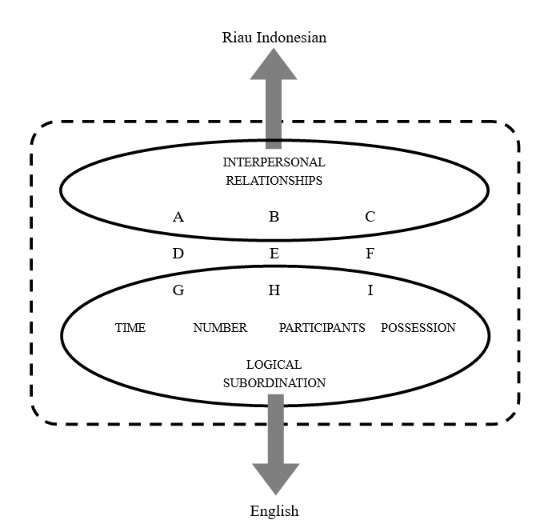
\includegraphics[width=0.8\textwidth]{gil_figure4.png}
\caption{\label{fig:gil:fig4}Linguistic Perspective in Riau Indonesian and English}
\end{figure}

In Figure \ref{fig:gil:fig4}, the area enclosed by the dashed line represents our conceptualization of reality.  Within it, represented in small caps, are a variety of individual aspects of our conceptualization of reality which may potentially be expressed in language.  While some of these aspects are the ones discussed above, a potentially much larger number of other aspects are suggested by the letters A - I.  The two ovals show how Riau Indonesian and English select different subsets of these variegated aspects of reality; they thus represent the contrasting linguistic perspectives of the two languages.  In particular, they capture the fact that even though both languages possess formal devices for the expression of logical subordination, actually using them to form multiple embeddings is something that speakers of English often do while speakers of Riau Indonesian typically do not.

The preceding discussion thus provides an answer to Jim Hurford's question posed at the beginning of this section, namely, what was meant by 'idiomaticity'.  In doing so, it underscores the fact that knowing a languages involves mastery not only of lexicon, phonetics, phonology, morphology, syntax, semantics and discourse/pragmatics, but, crucially, also linguistic perspective.  In particular, in order to be able to speak Riau Indonesian properly, it is not enough to know how to construct multiple embeddings; in addition, one must also know that the actual use of such multiple embeddings is, in almost all cases, inappropriate — it's just not the Riau Indonesian way of speaking.

\section{Quantitative Comparison}
It may reasonably be objected that it is unfair to compare a standardized language such as English with a colloquial variety such as Riau Indonesian.  After all, there is substantial evidence that within many a language, subordination occurs more frequently in higher registers than in lower ones, and in written as opposed to oral modalities \citep[and others]{givon1979understanding,deutscher2000syntactic,karlsson2009aorigin,karlsson2009bsyntactic}. Indeed, corpora of spoken English are also likely to contain constructions similar to the English rendition of (9), 'There was a child, right, he was chased by a dog, then there was a man who liked the dog, and the man got hit by Ali'. 

Nevertheless, abstracting away from such language-internal variation, English as a whole is much more tolerant of multiple embedding than Malay/Indonesian, the macro-language of which Riau Indonesian is just one typical exemplar.  In order to support this claim empirically, a rough and ready corpus study was conducted making use of Google searches.  In both English and Malay/Indonesian, Google searches produce material representative not only of a range of different dialects, but also of a variety of registers ranging from the colloquial language of social media to the more formal language of written works.  Thus, it is reasonable to believe that comparing the results of Google searches in English and Malay/Indonesian abstracts away not only from modality effects but also from the effects of language-internal register-governed variation; such searches may thus potentially offer a fair and well-founded comparison of the two languages.

Some results of a comparative corpus study of English and Malay/Indonesian are presented in Tables \ref{tab:first-english}-\ref{tab:second-malay} below:

\begin{table}
\caption{First Comparison: English}
\label{tab:first-english}
 \begin{tabularx}{.8\textwidth}{X rrrr}
 \lsptoprule
 he thinks he said & $13,840,000$ & {} \\
 he & $4,870,000,000$ & $7 x 10^{-4}$ \\
 thinks & $4,260,000,000$ & $9 x 10^{-4}$\\
 said & $4,560,000,000$ & $8 x 10^{-4}$\\
 \lspbottomrule
 \end{tabularx}
\end{table}

\begin{table}
\caption{First Comparison: Malay/Indonesian}
\label{tab:first-malay}
 \begin{tabularx}{.8\textwidth}{X rrrr}
 \lsptoprule
 dia pikir dia bilang & $7$ & {} \\
 dia (3\textsc{sg}) & $4,060,000,000$ & $2 x 10^{-9}$ \\
 pikir (think) & $38,000,000$ & $2 x 10^{-7}$\\
 bilang (say) & $1,210,000,000$ & $6 x 10^{-9}$\\
 \lspbottomrule
 \end{tabularx}
\end{table}

\begin{table}
\caption{Second Comparison: English}
\label{tab:second-english}
 \begin{tabularx}{.8\textwidth}{X rrrr}
 \lsptoprule
 he said he thinks & $10,200,000$ & {} \\
 he & $4,870,000,000$ & $2 x 10^{-3}$ \\
 thinks & $4,260,000,000$ & $2 x 10^{-3}$\\
 said & $4,560,000,000$ & $2 x 10^{-3}$\\
 \lspbottomrule
 \end{tabularx}
\end{table}

\begin{table}
\caption{Second Comparison: Malay/Indonesian}
\label{tab:second-malay}
 \begin{tabularx}{.8\textwidth}{X rrrr}
 \lsptoprule
 dia bilang dia pikir & $37,800$ & {} \\
 dia (3\textsc{sg}) & $4,060,000,000$ & $9 x 10^{-6}$ \\
 pikir (think) & $38,000,000$ & $1 x 10^{-3}$\\
 bilang (say) & $1,210,000,000$ & $3 x 10^{-5}$\\
 \lspbottomrule
 \end{tabularx}
\end{table}

Tables \ref{tab:first-english}-\ref{tab:second-malay} present two comparisons of English and Malay/Indonesian, the first in Tables \ref{tab:first-english} and \ref{tab:first-malay} and the second in Tables\ref{tab:second-english} and \ref{tab:second-malay}.  In Tables \ref{tab:first-english}-\ref{tab:second-malay}, the first column presents the search criterion, and the second column the rough number of hits (accessed on the 5th of June 2022).  Within each table, the first row presents a string, part of a complex construction which, when adding some following text, involves two levels of embedding, while the subsequent rows present the individual words occurring within the complex construction.

By examining the ratio of hits for the complex construction in the first line to that of the individual words in the subsequent lines, it is possible to abstract away both from the different sizes of the two corpora and also from possible frequency effects associated with the individual words, and in so doing measure the propensity of the language to form multiple embeddings making use of the words in question.  These ratios are presented in rounded form in the third column of each table.  For example, in Table \ref{tab:first-english}, the ratio of \emph{he} in line 2 to \emph{he thinks he said} in line 1 is $3,840,000 / 4,870,000,000 = 7 x 10^{-4}$.  On its own, this figure does not mean much; what is significant is its comparison to the corresponding figure in Table \ref{tab:first-malay}, in which the the ratio of \emph{dia} in line 2 to \emph{dia pikir dia bilang} in line 1 is $7 / 4,060,000,000 = 2 x 10^{-9}$.  Comparing these two figures, $7 x 10^{-4}$ and $2 x 10^{-9}$, shows that with respect to the particular words chosen, English is 4 to 5 orders of magnitude more likely to form the multiple embedding construction than Malay/Indonesian.  Comparable order-of-magnitude differences are present for the remaining five comparisons between Tables \ref{tab:first-english} and \ref{tab:first-malay}, and for five out of six of the corresponding comparisons between Tables \ref{tab:second-english} and \ref{tab:second-malay} — the only case where there is not a order-of-magnitude difference being in the third lines of Tables \ref{tab:second-english} and \ref{tab:second-malay}, where the English is ``only'' about twice as likely to form a multiple embedding construction than the Malay/Indonesian.

Thus, Tables \ref{tab:first-english}-\ref{tab:second-malay} show that English as a whole is massively more likely to form multiple embedding constructions than Malay/Indonesian.  In yet another comparison aimed at testing this generalization, the English string \emph{who do you think is going to win} yielded a total of $841,000$ hits, while there were no hits whatsoever for numerous potential equivalent sentences in Malay/Indonesian, the only exception being 3 hits for \emph{siapa anda pikir akan menang} (who 2 think FUT win), which actually occurred in an Indonesian website explaining the meaning of a similar English sentence — the exception that proves the rule.

The above Google searches show that multiple embedding is massively more common in English than in Malay/Indonesian.  The similar nature of the searches in the two languages shows that the greater propensity for subordination in English as compared to Malay/Indonesian is  a cross-linguistic difference that is independent of both register and modality.  In particular, the more widespread use of embedding in English is observable notwithstanding a significant body of literature \citep{karlsson2007aconstraints,karlsson2007bconstraints,karlsson2009aorigin,karlsson2009bsyntactic} showing that such constructions are more highly constrained, and occur less frequently in real live language use, than is commonly assumed to be the case under a simplistic characterization of English and other similar languages as syntactically recursive.

The results of the comparison between syntactic recursion in Malay/Indonesian and English is summarized in Figure \ref{fig:gil:fig5}:

\begin{figure}
\centering
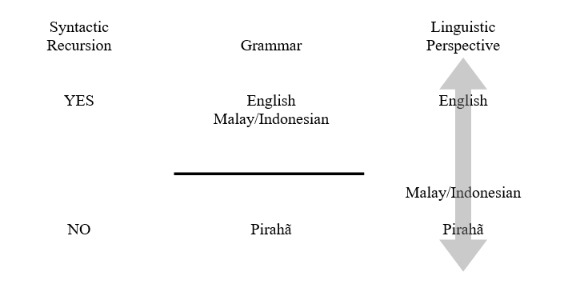
\includegraphics[width=0.8\textwidth]{gil_figure5.png}
\caption{\label{fig:gil:fig5}Recursion in Riau Indonesian and English}
\end{figure}

In terms of grammar, the distinction between having recursion and not having it is categorical; Malay/Indonesian (including Riau Indonesian) like English, has it, while Pirahã does not.  In contrast, with respect to linguistic perspective, the propensity for syntactic subordination and the use of recursive strategies to effect such subordination is a scalar property; while English makes frequent use of such embedding, Malay/Indonesian does not, though perhaps — this remains an open question — not to quite the same extent as Pirahã.  Thus, Figure \ref{fig:gil:fig5} shows why the question posed earlier, whether Riau Indonesian has syntactic recursion, is appropriately answered with a ``yes and no''.  Answering the question in this way underscores the importance, in any description of a language, not only of its lexicon and grammar, the things that one can say, but also of its linguistic perspective, the things that one actually does say.

\section{Towards a Cross-Linguistic Typology}

How do other languages fit into the above schema: are more languages like English, like Malay/Indonesian, or like Pirahã?  In addition, since linguistic perspective offers a scalar rather than a categorical take on recursion, there is also the potential for languages to occupy other points on the scale, possibly higher than English, or in-between English and Malay/Indonesian, with respect to their propensity for multiple embedding and their associated degrees of recursion.

At present, we simply do not know enough to provide a systematic answer to the above question.  Recursion is in the eyes of the beholder, with different analyses pointing towards alternative conclusions with regard to whether a given construction constitutes an instantiation of subordination or not.  If linguist A says that language X is syntactically recursive, while linguist B argues that language Y is not, then is this a real difference between the two languages, or merely a difference in the ways the two linguists choose to pursue their trade?  Indeed, for many individual languages, different linguists offer different answers to the question whether the language is syntactically recursive, as, we saw earlier with the contrasting analyses of Riau Indonesian offered by myself and by Jackendoff and Wittenberg. In fact, in some cases, it is not different linguists proposing different analyses but the same linguist modifying their views over time, an apparent instance of this being Dan Everett on Pirahã, as described in detail by Pullum (this volume).

As reflected by the evolution of Everett's writings on Pirahã, whether or not linguists choose to analyze a particular language as exhibiting syntactic recursion may be affected in a systematic fashion by their methodology, and, in particular, the relative weights that they attribute to data deriving from elicitation as opposed to naturalistic corpora.  In general, elicitation is more likely to lead to insights into grammar, and what people \emph{can} say, whereas work based on naturalistic corpora stands a greater chance of yielding a better understanding of linguistic perspective, and what people actually \emph{do} say.  Thus, elicitation, and asking speakers whether they would be willing to accept a long and unwieldy construction, is more conducive to the positing of syntactic recursion, whereas observation of naturalistic texts, in which such constructions may occur rarely, if at all, is more likely to lead to a claim to the effect that syntactic recursion is absent.  In particular, claims by scholars such as \citet{sandalo2018selfembedded}, and indeed for that matter also the early \citet{everett1986piraha}, to the effect that the grammar of Pirahã has at least some syntactic subordination, tend to be the products of elicited data, motivated by theoretical concerns, and as shown in detail by Pullum (this volume), a desire to fit the language into a predetermined descriptive template.  In contrast, the later and more famous claims by Dan Everett that Pirahã lacks syntactic recursion are mostly based on the use of naturalistic data.  While for Pirahã it may indeed be the case, as argued by Pullum (this volume), that the work based on elicitation is of inferior quality to the work based on naturalistic data, this is a contingent fact and not an inherent property of elicitation as opposed to the use of naturalistic corpora — there can be good or bad work based on elicitation just as there can be good or bad work making use of naturalistic data.  Thus, in view of the diverse methodologies underlying the available descriptions and analyses of different languages, it is not yet possible to paint a systematic picture of cross-linguistic variation with regard to syntactic recursion, but only to offer some observations and conjectures.

To begin with, one may ask whether there are languages in which syntactic recursion is even more prevalent than in English.  One phenomenon that comes to mind is that of clause chaining in many of the languages of New Guinea, as described by \citet{foley2010clause} and others.  In such languages, a sequence of several monoclausal sentences in English are rendered in the form of a single complex clause, in which all but the last of the clauses constitute a chain of embedded clauses marked by various morphosyntactic devices as subordinate.  However, as suggested by the term ``chaining'', the non-final clauses are all of equal status to one another, and therefore do not exhibit the kind of multiple embedding that is of concern to us here.

A perhaps more promising case is argued by \citet{cysouw2023hierarchical} to be provided by German, as illustrated by sentences such as the following (from \emph{Juristische Schulung, Zeitschrift für Studium und Referendariat}, 10/2012, Verlag C.H. Beck, p. 866; the English translation was provided by Boban Arsenijević with the assistance of DeepL Translate.):

\ea

Solange sich der Gläubiger noch durch die nachgeholte Leistung in Natur, ggf. ergänzt durch den Ersatz von Verzögerungs- und sonstigen Schäden, vollständig in die Lage versetzen lässt, in der er sich bei pflichtgemäßer Leistung befände, und die Leistung für den Schuldner weniger kostspielig ist als die Zahlung von Schadensersatz statt der Leistung, gibt es keinen Grund, dem Gläubiger von vornherein die Entscheidung zwischen Erfüllung in Natur und Schadensersatz zu überlassen und ihm zu erlauben, dem Schuldner durch die Wahl des Schadensersatzes den Kostenvorteil der Leistungserbringung zu nehmen.

'As long as the creditor can still be fully put in the position he would be in if he had performed dutifully, by the subsequent performance in nature, supplemented, if necessary, by the compensation for delay and other damages, and the performance is less costly for the debtor than the payment of damages instead of performance, there is no reason to leave the creditor the choice between performance in nature and damages from the outset and to allow him to deprive the debtor of the cost advantage by choosing the way of damage compensation.'

\z

According to \citet{cysouw2023hierarchical}, such sentences, complex to the point of unintelligibility for the average reader, are more common in German than in English.  To the extent that this observation holds water, it would seem to indicate that German may be characterized by a greater propensity for multiple embedding than English.  Some further discussion of stylistic variation with respect to the propensity for various kinds of subordination in the languages of Europe can be found in \citet{karlsson2007aconstraints, karlsson2007bconstraints}, suggesting, inter alia, that contemporary English might represent the outcome of recent processes of reduction in the extent to which such constructions, involving multiple embedding, are used.

At the other end of the scale represented in Figure \ref{fig:gil:fig5} are languages whose grammars do not allow syntactic recursion, or whose linguistic perspectives and associated patterns of usage disfavour it.  Again, one may ask whether and to what extent Malay/Indonesian and Pirahã are weird outliers, and the answer, surprising perhaps only to those whose primary concern is English and its representation within certain contemporary syntactic theories, is that they are not at all exceptional.  Thus, \citet[298]{givon1979understanding} writes that ``there are some languages extant to this day — all in preindustrial, illiterate societies with relatively small, homogenous social units — where one could demonstrate that subordination does not really exist  \ldots ''.  Givón's assertion is cited approvingly by \citet{pullum2010recursion} and Pullum (this volume), who go on to adduce several descriptions of languages reported as lacking subordination, among which are Amazonian languages such as Hixkaryana
\citep{derbyshire1979hixkaryana} and Apalaí \citep{koehn1986apalai}, Australian languages such as Dyirbal \citep{dixon1972dyirbal} and Wargamay \citep{dixon1981wargamay}, and various ancient languages, either attested, such as Old Akkadian \citep{deutscher2000syntactic}, or reconstructed, such as Proto-Uralic \citep{collinder1960comparative}.  And doubtlessly there are many more such languages, whose existence may been obscured by a common analytical bias that leads us to seek out complex structures where none actually exist.  Thus, with respect to syntactic recursion, at least, Pirahã is in good company, and is anything but some kind of strange outlandish creature, or, as intimated by some of Dan Everett's critics, something even worse than that.  Indeed, given the large number of languages still associated with such ``preindustrial, illiterate societies'', one is even led to wonder whether such languages might constitute the cross-linguistic norm.

And what of Riau Indonesian?  As suggested above, its extreme disfavouring of subordination is quite unexceptional; this is true not only within Malay/Indonesian (see \cite{englebretson2003searching} for a similar take on another colloquial variety of Indonesian, spoken on the island of Java) but also cross-linguistically. Nevertheless, the availability, however dispreferred,  of constructions such as that in \REF{ex:gil:1} shows that Riau Indonesian is not quite like Pirahã or any of the other languages cited above.  This rather extreme clash between what people can say and how people do actually speak is due, at least in part, to the much more complex sociolinguistic circumstances associated with Riau Indonesian, and other similar colloquial varieties of Malay/Indonesian. Such colloquial varieties of Malay/Indonesian occupy the bottom reaches of a lectal cline, at whose upper end are the two standardized versions of the language, Standard Indonesian and Standard Malay.  Although structurally quite distinct from one another, colloquial and standard versions of Malay/Indonesian are both present in the minds of diglossic speakers, and as a result, each of the two ends of the cline, colloquial and standard, exerts a substantial effect on its counterpart at the opposite end.  On the one hand, it is the presence of multiple embedding in Standard Indonesian that allows a speaker of Riau Indonesian to accept, however reluctantly, constructions such as that in \REF{ex:gil:1}, thereby supporting the characterization of Riau Indonesian grammar as syntactically recursive. In this respect, then, Riau Indonesian differs from Pirahã and other similar languages lacking a standardized acrolect that might be more conducive to such recursion.  On the other hand, it is the extreme disfavouring of subordination in Riau and other colloquial varieties of Indonesian that percolates upwards along the lectal cline, resulting in a relative disfavouring of subordination also in Standard Indonesian and Malay, as reflected by the differential results of the Google searches reported on in Section 4 earlier.  In this regard, Malay/Indonesian presents a clear contrast to English.  Standard Malay and Indonesian constitute special registers, not acquired natively by speakers through the usual processes of first language acquisition; they are thus parasitic on their colloquial counterparts. In contrast, Standard English is a more natural language variety that is indeed acquired natively by a large population of speakers, and is therefore relatively more resistant to influences from basilectal varieties of English, as, for example, might be manifest in the disfavouring of subordination.

The existence of cross-linguistic variation with respect to syntactic recursion and the proclivity for subordination raises the question what the determining factors might be that underlie such variation.  Givón, in the above-cited passage, alludes to ``preindustrial, illiterate societies with relatively small, homogenous social units'' — a plausible hypothesis, but one still in need of solid empirical cross-linguistic support.  As suggested earlier, a major challenge faced by any attempt to seek such support is that whether or not a language has syntactic recursion is very much dependent on how it is analyzed.  What is needed, therefore, is a common yardstick by which different languages can be uniformly and objectively assessed with respect to their relative proclivities for syntactic subordination.

\section{Cumulative Tales}
A simple rough and ready measure for the assessment of syntactic recursion across languages is provided by the analysis of an easily-identifiable genre of verbal art, namely cumulative tales (\cites[230—234]{thompson1946folktale}[522:536]{aarne1961types}).

A well-known example of a cumulative tale is the Jewish Passover song Had Gadya, mostly in Aramaic though with some Hebrew interspersed, shown below transcribed in accordance with a Modern Hebrew pronunciation, followed by an English translation (by Eve Levavi, in \emph{Haggadah for Pesah, an English translation}, hosted on the Open Siddur Project):

\ea

Veata hakadoš barux hu vešaħat lemalʔax hamavet,\\	
 dešaħat lešoħet,\\
 dešaħat letora,\\
 dešata lemaya,\\
 dexava lenura,\\
 desaraf leħutra,\\
 dehika lekalba,\\
 denašax lešunra,\\
 deaxla legadya,\\
 dezabin aba bitrey zuzey.\\

 'Then the Holy One, Blessed be He, came and slaughtered the angel of death,\\
 who slaughtered the butcher,\\
 who slaughtered the ox, \\
 that drank the water, \\
 that put out the fire, \\
 that burned the stick, \\
 that beat the dog, \\
 that bit the cat, \\
 that ate the goat, \\
 that my father bought for two zuzim.'

\z

In (11) above, the last verse is presented, containing a total of 10 clauses, of which the last 9, introduced by the Aramaic relativizer \emph{de-}, are embedded, each within the clause immediately preceding it, like a set of Matryoshka dolls.  

The clear and well-defined structural properties of cumulative tales provide an objective criterion enabling their cross-linguistic and cross-cultural distribution to be gauged.  In the absence — as far as I was able to determine — of any existing systematic cross-linguistic study of cumulative tales, a query was posted on the LINGTYP list (\url{https://listserv.linguistlist.org/pipermail/lingtyp/2023-February/thread.html}) in which its diverse readership, encompassing typologists familiar with a wide range of the world's languages, were asked if they were familiar with examples of cumulative  tales or songs from their respective regions of expertise.  The responses that came in demonstrated that cumulative tales are indeed widespread across the world's languages and cultures, but with a crucial qualification.  It turns out that the Had Gadya type, involving syntactic recursion, is apparently the exception, and that in most cases, the recursion is of a purely semantic nature, and is not reflected by syntactic subordination — the formal relationship between the successive clauses instead being one of parataxis, or flat chaining.  An instance of the latter state of affairs is provided by the following example from an Alemannic dialect of German (cited in 
\cite[65]{meier1851deutsche} and \cite[39]{newell1905passover}, and translated into English by Claudia Wegener):

\ea

Gestern haun i fegelt, I haun e Kreuzer gwonne;\\
De Kreuzer haun u 'r Mutterb gean,\\
Mutter hat mir Kerne gean,\\
Kerne haun i 'm Müller gean,\\
Müller hat mir Mehl gean,\\
Mehl haun i 'm Becke gean,\\
Beck¬e hat mir Wede gean,\\
Wede haun i 'm Vater gean,\\
Vater hat mir e Stöckle gean,\\
Stöckle haun i 'm Lehrer hean.\\
Lehrer hat mir Tatze hean  \ldots \\
 
'Yesterday I went bowling, I won a kreutzer;\\
The kreutzer I gave to my mother, \\
My mother gave me corn, \\
The corn I gave to the miller, \\
The miller gave me flour, \\
The flour I gave to the baker, \\
The baker gave me a bun, \\
The bun I gave to my father, \\
My father gave me a stick, \\
The stick I gave to my teacher, \\
My teacher hit my hand  \ldots ' \\

\z

Although in terms of its semantic structure, example (12) bears a close resemblance its predecessor in (11), in the Allemanic case there is no syntactic subordination, but instead a sequence of independent clauses, connected to each other by successive relationships of coreferentiality between the subject NP of each clause and the object NP of the clause preceding it.  Syntactically, then, rather than Matryoshka dolls, the clauses in (12) are like beads on a string.

While the results of the LINGTYP survey cannot be considered more than preliminary, the emerging picture is one in which cumulative tales involving parataxis, as in example (12), are of widespread distribution, occurring in a variety of unrelated languages and cultural regions, and hence not accountable for in terms of a single ancestral case subsequently spreading by means of vertical inheritance or horizontal diffusion.  Some of the languages in which such syntactically flat cumulative tales are attested include Laal, an isolate language of southern Chad (Florian Lionnet p.c.); the Timimoun dialect of Arabic (\cite{mammeri1985ahellil}, Lameen Souag p.c.), Basque (Peter Bakker p.c.), the Nakh-Daghestanian language Agul (Timor Maisak p.c.), Tamil (Siva Kalyan p.c.), three at best distantly related languages of New Guinea, Pa, Northeastern Kiwai and Asmat \citep{voorhoeve2010remarkable}, and Yucatec Maya (\cite[180—186]{smailus1975textos}, Jürgen Bohnemeyer p.c.).  In contrast, no examples emerged of syntactically recursive cumulative tales, as in (11), from outside the Middle-Eastern / North African / European cultural area — even though, in many such languages, syntactic recursion is permitted by the grammar, and at least some syntactic subordination is used in ordinary speech.  

If indeed the limited distribution of syntactically recursive cumulative tales is found to hold up under more extensive empirical scrutiny, then this would potentially point towards one or both of the following two hypotheses governing their distribution.  The first hypothesis is diachronic:  In accordance with this hypothesis, all cases of syntactically recursive cumulative tales can be traced back to a single common origin, with their current distribution the outcome of an interplay of vertical inheritance and horizontal diffusion.  While it is beyond doubt that literary genres such as cumulative tales do indeed spread across time and space, what is at issue is whether such diachronic processes are the whole story, or whether other factors might also play a role in the observed distribution of syntactically recursive cumulative tales.  

The second hypothesis offers one such factor of a sociolinguistic orientation, appealing to the covariance of societal and grammatical complexity.  Following this hypothesis, the occurrence of syntactically recursive cumulative tales correlates positively with the complexity of the society with which it is associated, as measured by any of a number of potential yardsticks, in accordance with \citet{chen2023linguistic}.  In alternative formulations of the hypothesis, syntactically recursive cumulative tales would be more likely to occur in exoteric as opposed to esoteric societies \citep{thurston1987processes, wray2007consequences}; societies characterized as Western, Educated, Industrialized, Rich and Democratic, or WEIRD \citep{henrich2010weirdest, henrich2020weirdest}  or as Literate, Official, and with Lots of speakers, or LOL \citep{dahl2015weird}; societies high on Ethnologue's Expanded Graded Intergenerational Disruption Scale, or EGIDS \citep{eberhard2020ethnologue}; and societies of greater complexity as reflected in a variety of features in the D-PLACE database \citep{kirby2016dplace}, such as, for example, population size, population density, and the number of jurisdictional levels above the local community.  While the results of the informal LINGTYP survey are consistent with this hypothesis, more work is necessary before such a hypothesis can be empirically supported.

\section{Conclusion}

However interesting in its own right, the examination of the distribution of syntactically recursive cumulative tales is of course intended here as a mere proxy for a more general investigation into the cross-linguistic distribution of syntactic recursion.  While much harder to ascertain in an objective systematic manner, there is good reason to believe that the distribution of syntactic recursion more generally may be sensitive to the variegated aspects of societal complexity alluded to in the second hypothesis above.  That is to say, syntactic recursion is more likely to be found in societies of greater complexity. 

One centrally important aspect of societal complexity mentioned earlier is modality.  As already noted, syntactic recursion is more commonly found in writing than in speech; moreover, this tendency may be manifest in two distinct ways, online and conventionalized. To begin with, multiple embedding and associated syntactic recursion are more likely to occur in writing than in speech within a single language or even speaker.  But in addition, within the same modality, languages with an overall higher rate of literacy are more likely to make use of multiple embedding and allow syntactic recursion.  Evidence for this latter correlation was provided earlier by the contrasting results of the Google searches in English, with a higher rate of literacy, and Malay/Indonesian, which, as suggested in \citet[30]{gil2009grammar}, is characterized by a lower rate of literacy and correspondingly lower functional range of written communication.

Nevertheless, literacy is just one of an array of features generally associated with societal complexity, and there is good reason to believe that several of these other features may also be associated with a greater propensity for recursion.  A series of recent studies have demonstrated positive correlations between various aspects of societal and linguistic complexity.  Thus, recent experiments by \citet{raviv2019larger,raviv2020role} and \citet{raviv2020language} show that in artificial languages, larger speech communities entail more conventionalization, which is tantamount to greater grammatical complexity. Similarly, in sign languages, \citet{meir2012influence, ergin2020community} argue that an increase in the size of the signing community entails a greater degree of conventionalization.  In phonology, \citet{hay2007phoneme,atkinson2011phonemic,wichmann2011phonological,nettle2012social} argue that larger languages tend to have larger phonemic inventories than smaller languages. In the domain of metaphor comprehension, \citet{gil2021metaphors} present evidence to the effect that more highly complex polities tend to be associated with languages whose metaphors are of more complex directional structure.  With respect to Tense-Aspect-Mood marking, \citet{gil2021tense} demonstrates that languages belonging to larger families, the product of demographic spread, are associated with more complex systems characterized by obligatory as opposed to optional marking.  Finally, in the realm of basic clause structure, work in progress, some initial results of which are summarized in \citet{gil2019grammar}, shows that more highly complex polities tend to be associated with languages endowed with a greater degree of grammaticalization of thematic-role assignment.  Admittedly, though, a range of other studies support an opposite negative correlation between societal and linguistic complexity.  As argued by \citet{mcwhorter2018creole,mcwhorter2005defining,mcwhorter2011linguistic,dahl2004growth,wray2007consequences,lupyan2010language,trudgill2011sociolinguistic} and others, larger political entities, typically associated with various modes of exoteric communication, and in particular imperfect adult second-language acquisition, are conducive to linguistic simplification, whereas smaller societies, generally characterized by more esoteric forms of communication, are fertile grounds for the accretion of linguistic complexity.  A way of reconciling these apparently divergent results is proposed in \citet{chen2023linguistic}, who demonstrate, in a quantitative study based on data from the World Atlas of Language Structures, or WALS \citep{haspelmath2005atlas}, that many of the linguistic features associated with a positive correlation between linguistic and societal complexity tend to be of a syntactic nature; in addition, they speculate that such features will tend to rely more on procedural as opposed to declarative memory. Since recursion was not included in the features examined in WALS, it is not mentioned in the \citet{chen2023linguistic} study.  However, the generalizations emerging from that study strongly suggest that, as manifestations par excellence of syntactic complexity, syntactic subordination and recursion should also exhibit a positive correlation with societal complexity.

Viewed in the light of the covariance of societal and syntactic complexity, the facts regarding recursion in Malay/Indonesian, Pirahã and English, as summarized in Figure \ref{fig:gil:fig5}, make perfect sense.  In terms of societal complexity, Malay/Indonesian occupies an intermediate position between Pirahã and English.  Whereas Pirahã is spoken by a single small group of people with relatively little contact with the outside world, Malay/Indonesian, in all of its varieties, is spoken by well over two hundred million people and is an official language of four different countries.  No wonder, then, that, unlike Pirahã, Malay/Indonesian allows for syntactic recursion, a fact that is true also for colloquial varieties such as Riau Indonesian.  However, in contrast to Malay/Indonesian, English is a world language, a vehicle not only of national but also international communication; moreover, unlike Malay/Indonesian, its standardized versions are spoken natively by large populations of speakers.  It is this difference that accounts for the massively greater frequency of subordination, a reflection of syntactic recursion, in actual English usage, as contrasted with Malay/Indonesian.

\section*{Abbreviations}
\begin{tabularx}{.5\textwidth}{@{}lQ@{}}
\textsc{assoc} & associative \\
\textsc{hyp} & hypocoristic \\
\textsc{prtc} & participant \\
\end{tabularx}

\section*{Acknowledgements}
It is a pleasure to dedicate this paper to Dan Everett, in some ways a kindred soul.  I am also grateful to Ted Gibson for inviting me to be part of this festschrift.  For discussions of some of the issues dealt with in this paper I am indebted to Jim Hurford, Ray Jackendoff and Eva Wittenberg.  Thanks are due also to Caleb Everett for his comments on an earlier draft.  Some of the material in this paper was presented at the International Symposium on Malay/Indonesian Linguistics (ISMIL), in the 14th meeting in Minneapolis on 30 April 2010, the 19th meeting in Jambi on 2015, and at the 26th meeting in Honolulu on 19 May 2023; I am grateful to participants at those events for helpful comments and criticisms.  Finally, the work reported on here would not have been possible without the generous support of the Department of Linguistics of the Max Planck Institute of Evolutionary Anthropology and its director Bernard Comrie.

\printbibliography[heading=subbibliography,notkeyword=this]
\end{document}
